\section{SOH and RUL on ageing datasets}
\label{sec:aging}
The CALCE files cannot support SOH or RUL (Section~\ref{sec:results}). To exercise these modules, three downloaded CSV files were audited and used. \textbf{Their provenance differs and is kept separate throughout}: (i) \texttt{features\_arrhenius\_tempmean.csv}: battery IDs follow NASA naming and per-cycle features were computed by an unknown third party; we call it ``experimental-derived'' and its provenance is \emph{not verified}; (ii) \texttt{augmented\_full\_dataset.csv}: the same original rows plus three artificial replicas per battery; (iii) \texttt{pybamm\_synthetic\_features.csv}: a PyBaMM \emph{simulation} of six virtual batteries.

\subsection{Audit and definitions}
Table~\ref{tab:agingaudit} shows the rule-based exclusion of two batteries: one holds a single cycle, and one has a capacity reaching 2.6 times its first-cycle value (corrupted trajectory). Seven NASA-style batteries remain (two at 24\,°C, five at 4\,°C; initial capacities 1.08--2.04\,Ah, so no common nominal capacity exists). SOH is therefore defined \emph{relative to the cell's own first-cycle capacity}, $\mathrm{SOH}_{\mathrm{rel}}=Q/Q_1\times100$, \emph{not} to a nominal capacity. The files' own RUL labels were verified to correspond to the first cycle with $Q\le0.70\,Q_1$ (reproduced exactly for all 13 usable batteries), and $\mathrm{RUL}=N_{\mathrm{EOL}}-N$ is expressed in \emph{retained records}: the \texttt{cycle} column indexes retained records whose raw cycle positions are spaced by 2--4. The 70\,\% rule is not the 80\,\% convention mentioned in the project brief; it is the one the data support.
\begin{table}[htbp]\centering\footnotesize
\begin{tabular}{lrrrrr}
\toprule
 & Cycles & Q$_1$ (Ah) & max/first & Ambient (°C) & Usable \\
Battery &  &  &  &  &  \\
\midrule
B0005 & 162 & 1.86 & 1.00 & 24.00 & True \\
B0006 & 102 & 2.04 & 1.00 & 24.00 & True \\
B0033 & 1 & 0.69 & 1.00 & 24.00 & False \\
B0040 & 46 & 0.67 & 2.57 & 24.00 & False \\
B0041 & 22 & 1.22 & 1.00 & 4.00 & True \\
B0045 & 17 & 1.08 & 1.00 & 4.00 & True \\
B0046 & 41 & 1.73 & 1.00 & 4.00 & True \\
B0047 & 41 & 1.67 & 1.00 & 4.00 & True \\
B0048 & 52 & 1.66 & 1.00 & 4.00 & True \\
\bottomrule
\end{tabular}
\caption{Rule-based audit of the NASA-style batteries (exclusion: fewer than 15 cycles, or capacity above 115\,\% of the first cycle).}\label{tab:agingaudit}
\end{table}

\paragraph{Leakage control.} \texttt{RUL}, \texttt{NRUL} and \texttt{battery\_life} are answers; \texttt{capacity\_norm}, \texttt{capacity\_diff} and \texttt{capacity\_ma5} derive from capacity with an unknown normalisation; \texttt{arrhenius\_fade\_rate} is an exact function of \texttt{temp\_mean} ($R^2=1.0000$ in $\log$ rate versus $1/T$). None is used as input (enforced by a guard and unit tests). \texttt{Rct}/\texttt{Re} are constant and back-filled before the first measurement (look-ahead), so they appear only in an exploratory ablation. History features at cycle $k$ use cycles $\le k$ only. The artificial replicas are added only to the training rows of training batteries and never to any test set.

\subsection{Protocols}
Leave-one-battery-out (LOBO): the test battery is never seen in training or in the inner leave-one-battery-out tuning of the Random Forest grid. Temperature transfer: train on the two 24\,°C batteries and test on each 4\,°C battery, and conversely. Ambient temperature labels come from the file. Baselines for RUL: mean training life minus current cycle, and a causal linear extrapolation of $\mathrm{SOH}_{\mathrm{rel}}$ to the 70\,\% level (capped at the longest training life). RUL is evaluated from cycle~5 on.

\subsection{Results on the NASA-style (experimental-derived) data}
\begin{table}[htbp]\centering\footnotesize
\begin{tabular}{lllrrrrr}
\toprule
 &  &  & Batt. & MAE & RMSE & R$^2$ & MaxAE \\
Data & Features & Model &  &  &  &  &  \\
\midrule
\multirow[t]{4}{*}{NASA-style} & \multirow[t]{2}{*}{base} & random\_forest & 7 & 3.38 & 4.13 & 0.80 & 10.24 \\
 &  & linear & 7 & 6.07 & 7.39 & 0.36 & 26.06 \\
\cline{2-8}
 & \multirow[t]{2}{*}{cycle only} & linear & 7 & 8.81 & 10.05 & -0.19 & 18.93 \\
 &  & random\_forest & 7 & 9.00 & 10.45 & -0.29 & 21.45 \\
\cline{1-8} \cline{2-8}
\multirow[t]{4}{*}{PyBaMM (sim.)} & \multirow[t]{2}{*}{cycle only} & linear & 6 & 1.60 & 2.16 & 0.93 & 6.15 \\
 &  & random\_forest & 6 & 1.62 & 2.14 & 0.93 & 6.58 \\
\cline{2-8}
 & \multirow[t]{2}{*}{base} & random\_forest & 6 & 1.89 & 2.35 & 0.92 & 5.62 \\
 &  & linear & 6 & 3.52 & 4.41 & 0.72 & 11.03 \\
\cline{1-8} \cline{2-8}
\bottomrule
\end{tabular}
\caption{SOH leave-one-battery-out, pooled over held-out batteries (SOH points). ``PyBaMM (sim.)'' rows are \emph{simulated} data.}\label{tab:tab_aging_soh}
\end{table}

SOH (Table~\ref{tab:tab_aging_soh}, Fig.~\ref{fig:soh}): Random Forest with the per-cycle signal features reaches a pooled MAE of 3.4 SOH points ($R^2=0.80$), against 6.1 for linear regression; the cycle index alone is inadequate ($R^2<0$) because battery lives range from 17 to 162 records. Features such as incremental-capacity and voltage statistics derive from the same discharge as the capacity, so this is an estimation of capacity from curve features, not an independent validation.
\begin{figure}[H]\centering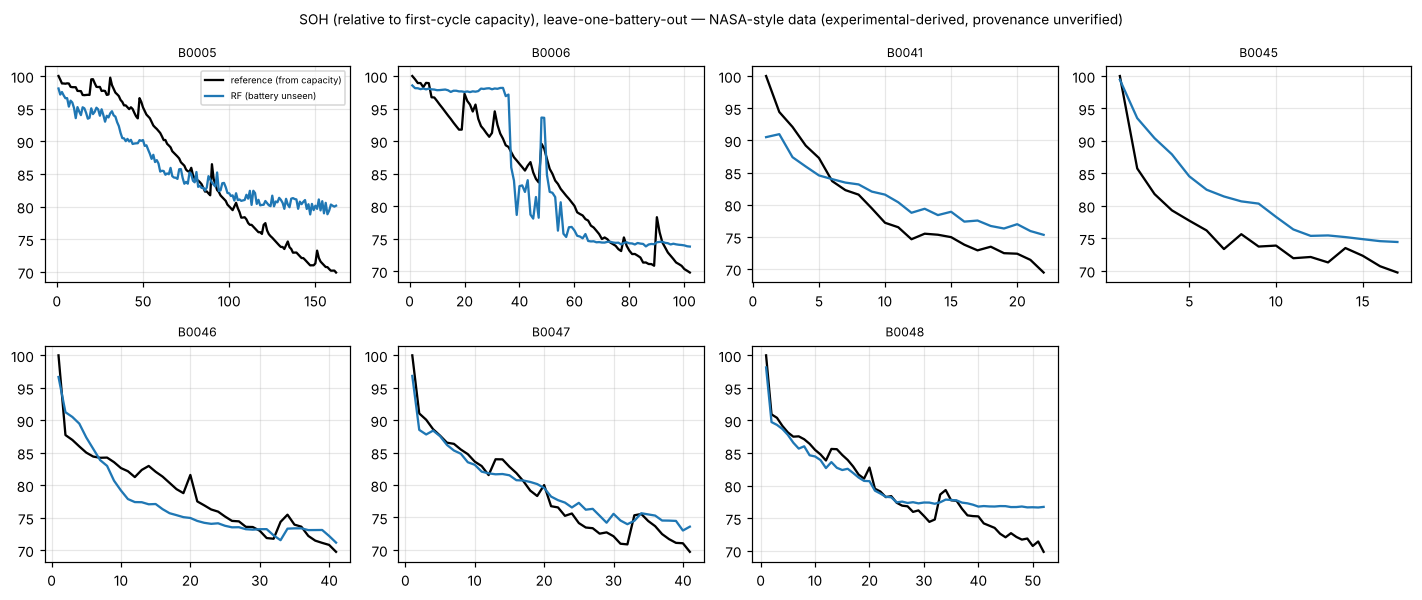
\includegraphics[width=\linewidth]{fig11_aging_soh_nasa_lobo.png}\caption{SOH (relative to first cycle), Random Forest, battery unseen. NASA-style data.}\label{fig:soh}\end{figure}
\begin{table}[htbp]\centering\footnotesize
\begin{tabular}{lllrrrrr}
\toprule
 &  &  & Batt. & MAE & RMSE & R$^2$ & MaxAE \\
Data & Features & Model &  &  &  &  &  \\
\midrule
\multirow[t]{6}{*}{NASA-style} & \multirow[t]{2}{*}{capacity history} & linear & 7 & 17.14 & 23.74 & 0.68 & 76.31 \\
 &  & random\_forest & 7 & 19.90 & 26.79 & 0.59 & 62.37 \\
\cline{2-8}
 & history+signals & random\_forest & 7 & 20.08 & 29.29 & 0.51 & 73.88 \\
\cline{2-8}
 & capacity history & baseline\_linear\_extrap & 7 & 26.20 & 37.38 & 0.20 & 156.00 \\
\cline{2-8}
 & history+signals & linear & 7 & 34.56 & 42.07 & -0.01 & 66.09 \\
\cline{2-8}
 & capacity history & baseline\_mean\_life & 7 & 46.35 & 57.50 & -0.88 & 116.17 \\
\cline{1-8} \cline{2-8}
\multirow[t]{6}{*}{PyBaMM (sim.)} & \multirow[t]{2}{*}{capacity history} & random\_forest & 6 & 7.22 & 10.50 & 0.96 & 46.21 \\
 &  & linear & 6 & 9.11 & 12.72 & 0.95 & 41.17 \\
\cline{2-8}
 & history+signals & random\_forest & 6 & 15.22 & 19.62 & 0.87 & 52.37 \\
\cline{2-8}
 & \multirow[t]{2}{*}{capacity history} & baseline\_linear\_extrap & 6 & 16.13 & 19.82 & 0.87 & 65.77 \\
 &  & baseline\_mean\_life & 6 & 18.40 & 22.74 & 0.83 & 42.00 \\
\cline{2-8}
 & history+signals & linear & 6 & 43.92 & 50.04 & 0.17 & 106.48 \\
\cline{1-8} \cline{2-8}
\bottomrule
\end{tabular}
\caption{RUL leave-one-battery-out, pooled over held-out batteries (records). ``PyBaMM (sim.)'' rows are \emph{simulated} data.}\label{tab:tab_aging_rul}
\end{table}

RUL (Table~\ref{tab:tab_aging_rul}, Fig.~\ref{fig:rulnasa}): the best pooled MAE is 17.1 records (linear regression on capacity-history features, $R^2=0.68$), then Random Forest at 19.9, the linear-extrapolation baseline at 26.2 and the mean-life baseline at 46.4 ($R^2<0$). Adding the signal features \emph{degrades} both models (linear: 34.6). Relative to the battery life the errors are large for the short-lived batteries (per-battery MAE of 6--45\,\% of life for the Random Forest and 12--74\,\% for linear regression). The Random Forest cannot predict beyond the longest training life: with B0005 (162 records) held out, its predictions saturate near 100 (Fig.~\ref{fig:rulnasa}). The 5--95\,\% spread of the trees is a heuristic, not a calibrated interval: it contains the true RUL for only 54\,\% of the points on average (nominal 90\,\%).
\begin{figure}[H]\centering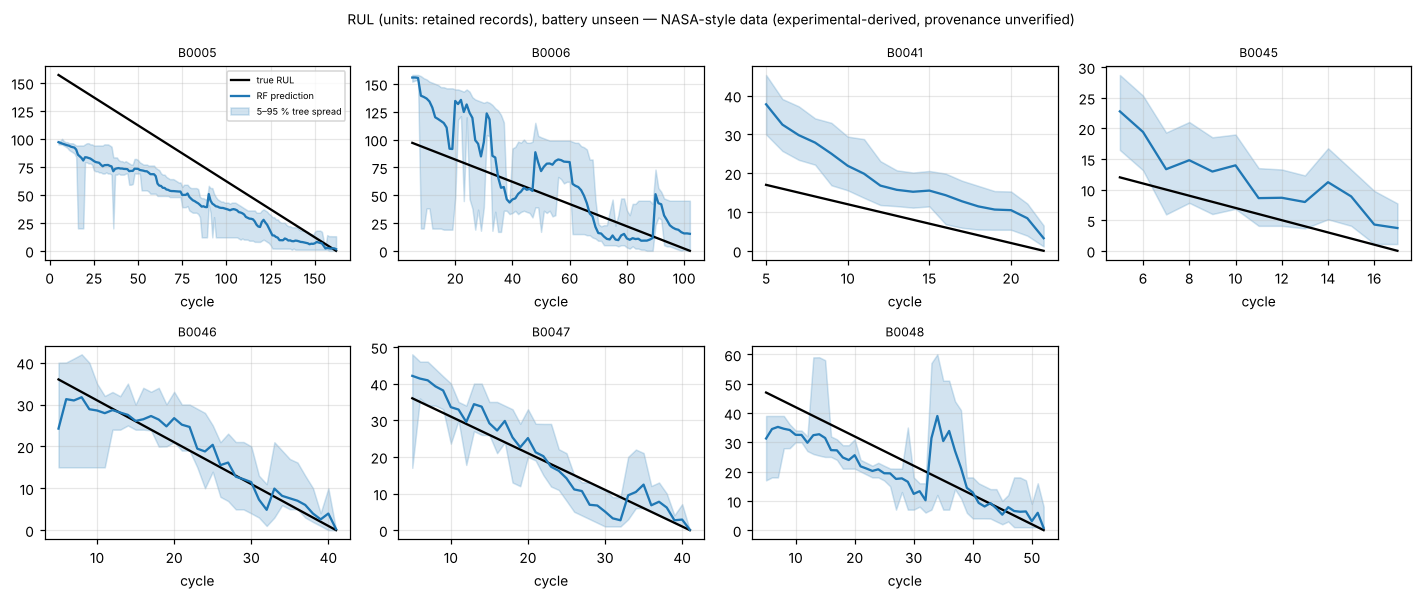
\includegraphics[width=\linewidth]{fig12_aging_rul_nasa_lobo.png}\caption{RUL (retained records), Random Forest on capacity-history features, battery unseen. NASA-style data.}\label{fig:rulnasa}\end{figure}
\begin{table}[htbp]\centering\footnotesize
\begin{tabular}{llllrrrr}
\toprule
 &  &  &  & Batt. & MAE & RMSE & R$^2$ \\
Target & Protocol & Features & Model &  &  &  &  \\
\midrule
\multirow[t]{10}{*}{RUL} & \multirow[t]{4}{*}{cross\_temperature\_24to4} & capacity history & linear & 5 & 12.21 & 14.71 & -0.42 \\
\cline{3-8}
 &  & history+signals & linear & 5 & 26.29 & 30.14 & -4.98 \\
\cline{3-8}
 &  & capacity history & random\_forest & 5 & 19.48 & 21.81 & -2.13 \\
\cline{3-8}
 &  & history+signals & random\_forest & 5 & 12.17 & 13.72 & -0.24 \\
\cline{2-8} \cline{3-8}
 & \multirow[t]{4}{*}{cross\_temperature\_4to24} & capacity history & linear & 2 & 40.79 & 49.65 & -0.37 \\
\cline{3-8}
 &  & history+signals & linear & 2 & 44.16 & 54.51 & -0.65 \\
\cline{3-8}
 &  & capacity history & random\_forest & 2 & 43.99 & 56.19 & -0.75 \\
\cline{3-8}
 &  & history+signals & random\_forest & 2 & 38.03 & 48.84 & -0.32 \\
\cline{2-8} \cline{3-8}
 & \multirow[t]{2}{*}{lobo\_with\_augmented\_training\_rows} & \multirow[t]{2}{*}{history+signals} & linear & 7 & 34.59 & 42.11 & -0.01 \\
 &  &  & random\_forest & 7 & 22.26 & 31.70 & 0.43 \\
\cline{1-8} \cline{2-8} \cline{3-8}
\multirow[t]{6}{*}{SOH} & \multirow[t]{2}{*}{cross\_temperature\_24to4} & \multirow[t]{2}{*}{base} & linear & 5 & 3.79 & 4.99 & 0.47 \\
 &  &  & random\_forest & 5 & 5.50 & 6.73 & 0.03 \\
\cline{2-8} \cline{3-8}
 & \multirow[t]{2}{*}{cross\_temperature\_4to24} & \multirow[t]{2}{*}{base} & linear & 2 & 6.16 & 7.17 & 0.47 \\
 &  &  & random\_forest & 2 & 8.21 & 9.45 & 0.07 \\
\cline{2-8} \cline{3-8}
 & \multirow[t]{2}{*}{lobo\_with\_augmented\_training\_rows} & \multirow[t]{2}{*}{base} & linear & 7 & 6.14 & 7.46 & 0.34 \\
 &  &  & random\_forest & 7 & 3.17 & 3.89 & 0.82 \\
\cline{1-8} \cline{2-8} \cline{3-8}
\bottomrule
\end{tabular}
\caption{NASA-style data: temperature transfer (24\,°C$\leftrightarrow$4\,°C) and augmentation ablation.}\label{tab:agingtransfer}
\end{table}

Temperature transfer and augmentation (Table~\ref{tab:agingtransfer}): no successful cross-temperature generalisation was obtained. $R^2$ never exceeds 0.47 for SOH and is negative for every RUL model; the 24\,°C$\rightarrow$4\,°C direction rests on only two training batteries and the reverse on two test batteries. Adding artificial replicas of the training batteries brings no consistent gain (Random Forest SOH MAE 3.4$\rightarrow$3.2; RUL 20.1$\rightarrow$22.3), consistent with replicas carrying no new information.

\subsection{Results on the simulated PyBaMM data}
\emph{These results are simulated and are not experimental evidence.} Cycle index alone gives $R^2=0.93$ for SOH (MAE 1.6 points) and the signal features do not improve it, which shows that the virtual batteries age in nearly identical ways. Random Forest on capacity-history features reaches an RUL MAE of 7.2 records ($R^2=0.96$) against 16.1 and 18.4 for the baselines. This indicates that the pipeline works on well-behaved data; it says nothing about real batteries.

\subsection{Interpretation and limits}
Seven batteries from two ambient temperatures give low statistical power: pooled metrics are dominated by the longest-lived batteries, and the ranking of models could change with other cells. SOH here is relative to the first cycle, EOL follows the dataset's 70\,\% rule, RUL is in records, and the provenance of the features is unverified. Conclusions are limited to: (i) the pipeline respects leakage and battery-level separation, (ii) on the experimental-derived data, capacity-history features support a moderately accurate RUL and signal features support SOH, (iii) temperature transfer and augmentation were not shown to help.
